\setlength{\footskip}{8mm}

\chapter{Introduction} 

\textit{This dissertation explores the possibilities and develops
algorithms for modeling human behaviors and detecting anomalies
without requiring large databases of training data. In this chapter, I
discuss the background and motivation of my work, review real-world
surveillance systems, present the contributions of the work, and
provide an outline of this dissertation.}

\section{Background and Motivation}

Due to the increase in demand for video surveillance in public areas,
video surveillance is becoming ubiquitous in our lives. It becomes
increasingly important for preventing and responding to terrorist and
other criminal activities. However, the resulting proliferation of
surveillance cameras is making it increasingly difficult to monitor
all channels continuously. Human monitoring is therefore becoming
increasingly expensive and ineffective as the torrent of video data
increases. For instance, in a CCTV monitoring room (see
Figure \ref{fig:monitoring}), security operators are required to
monitor 24 hours a day and be ready to take action when an alarm
occurs. Security will be enhanced if there is an intelligent
surveillance system able to perform filtering, archiving ``normal''
events, and automatically raising alarms for possible ``abnormal''
events or presenting such events to human security personnel for
consideration as a security threat. The problems to consider in a
surveillance system include pedestrian detection and tracking,
unattended object detection, human behavior modeling, and anomaly
detection.

\begin{figure}[t]
    \centering
    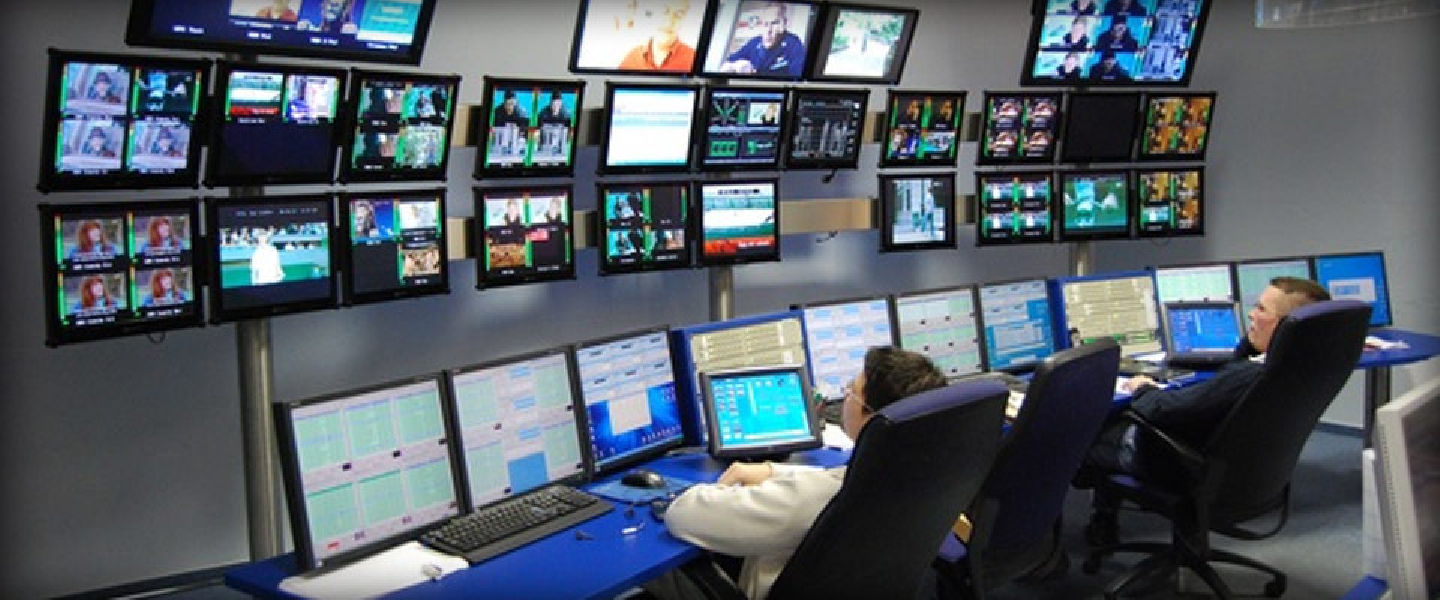
\includegraphics[width=5in]{figures/monitoring}
    \caption[CCTV monitoring room.]{\small CCTV monitoring
        room. Reprinted from the Twenty First Security Web site
        (\url{http://www.twentyfirstsecurity.com.au/}).}
    \label{fig:monitoring}
\end{figure}

Human behavior understanding is one of the key components of
intelligent video surveillance. However, the problem is difficult and
remains unsolved, due to the wide range of activities possible in any
given context and the large amount of variability within any
particular activity.

One limitation of much of the existing work is that it learns in batch
mode and creates separate models, which remain static once trained,
for each distinct class of behavior. It may have an advantage in
explaining data that are well-defined, but it needs sufficiently large
samples of behavior patterns before training the system. Another
limitation is that the number of ``normal'' behavior patterns needs to
be known beforehand because we cannot learn a model for ``abnormal''
behavior that is rare and diverse. Therefore, we must instead detect
deviations from typical behavior.

The ambiguity of human behaviors makes the problem more challenging
since it is scene-dependent and can change over time. In particular, a
behavior considered normal in one context might be considered unusual
in another context depending on the type of behavior and where and
when it is observed. The characteristics of typical behavior also vary
from scene to scene.

Many researchers have attempted to build surveillance systems able to
interpret and understand human behaviors. However, most of the work
learns behaviors in an offline fashion and keeps the model static once
trained. This is impractical for real-time surveillance applications,
since offline training requires a great deal of computational time and
resources. In addition, the number of behaviors needs to be known
beforehand. We therefore need to find a way to initially recognize and
model each of the common behavior groups in a particular scene as well
as to incrementally learn scene-specific models as new behavior is
observed.

Many open source and commercial video surveillance products are 
available. Most of the products do not implement any intelligent
features; therefore, they cannot learn and understand the events
occurring in a scene. Moreover, a great deal of configuration must be done
before a user can deploy the system to operate in a real situation.
For instance, a user may need to define restricted zones or rules
for a specific scene.

Three main challenges for human behavior understanding and anomaly
detection are as follows.

\begin{enumerate}
    \item It is impractical to store all data in a system; therefore, we
        need an efficient approach that learns scene-specific statistical
        models of human behavior without requiring storage of large
        databases of training data.
    \item Real human behavior is sometimes ambiguous; therefore, we need to 
        keep humans such as security personnel in the loop to interpret it.
    \item Unusual behavior is rare and diverse, and it is also impractical 
        to acquire sufficient data for a good model for it; therefore, we 
        need to detect deviations from typical behavior instead.
\end{enumerate}

In this dissertation, we propose to explore, implement, and evaluate
an efficient method for automatic identification of suspicious
behavior in video surveillance data that incrementally learns
scene-specific statistical models of human behavior without requiring
storage of large databases of training data. The method is based on
hidden Markov models (HMMs) with sufficient statistics and an optimal
threshold on the likelihood of an event according to the human
behavior model.  We begin by building an initial set of models
explaining the behaviors occurring in a small bootstrap data set. The
bootstrap procedure partitions the bootstrap set into clusters then
assigns new observation sequences to clusters based on statistical
tests of HMM log likelihood scores. Cluster-specific likelihood
thresholds are learned rather than set arbitrarily. After
bootstrapping, each new sequence is used to incrementally update the
sufficient statistics of the HMM it is assigned to. Our method is an
effective solution to the problem of inducing scene-specific
statistical models useful for bringing suspicious behavior to the
attention of human security personnel.

\section{Review of Real-World Surveillance Systems}

We divide this section into open source and commercial products.

\subsection{Open Source Products}

ZoneMinder (ZM; Coombes, 2007)\nocite{zoneminder} is an open source
video surveillance system for Linux. It has been released under the
terms of the GNU general public license (GPL). ZM supports both IP
cameras and USB cameras. Figure \ref{fig:zm-webcam} shows an example
of a scene captured by an IP camera and a USB camera. The system
consists of many independent modules including motion detection.  Each
component is designed to use as few resources as possible, maximizing
the efficiency of the machine. It provides a PHP-based Web interface
that allows us to control the cameras and monitor a scene from
anywhere. Besides controlling and monitoring, we can also review,
archive, or delete the events through its Web interface.

\begin{figure}[t]
  \begin{center}
    \subfloat[]{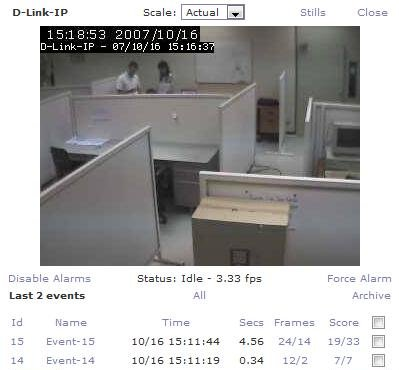
\includegraphics[scale=0.6]{figures/zm-webcam01.jpg}
    \label{fig:zm-webcam01}}
    \hspace{0.1in}
    \subfloat[]{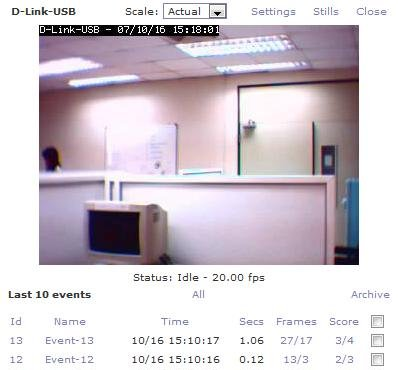
\includegraphics[scale=0.6]{figures/zm-webcam02.jpg}
    \label{fig:zm-webcam02}}
  \end{center}
  \caption[Example of a scene captured by ZoneMinder.]{\small Example
    of a scene captured by (a) an IP camera and (b) a USB camera from
    ZoneMinder.}
  \label{fig:zm-webcam}
\end{figure}

SecureCam \shortcite{bedecs09securecam} is a open source software for
Windows platform providing a friendly user interface as shown in
Figure \ref{fig:securecam}. Similar to ZoneMinder, SecureCame supports
multiple cameras and provides a few simple and fast algorithms such as
motion detection. It has e-mail and sound notification features, and
it also allows users to record video for later review.

\begin{figure}[t]
  \begin{center}
    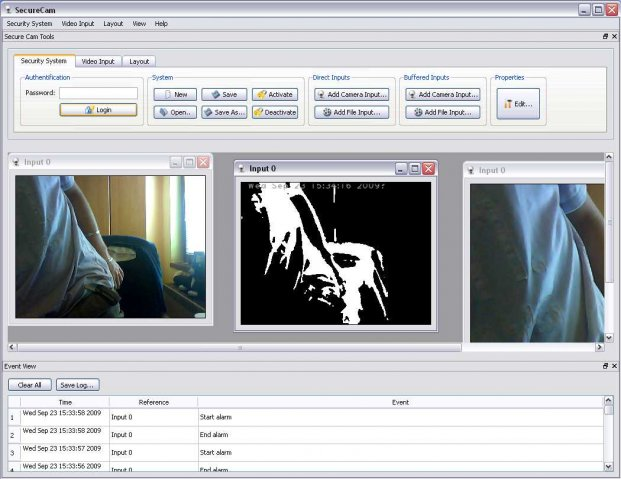
\includegraphics[width=4in]{figures/securecam.jpg}
    \caption[Screen shot of SecureCam.]{\small Screen shot of
      SecureCam. Reprinted from the SecureCam Web site
      (\url{http://sourceforge.net/projects/securecam/}).}
    \label{fig:securecam}
  \end{center}
\end{figure}

\subsection{Commercial Products}

Vitamin D Video \shortcite{vitamind} is a commercial video
surveillance system. It supports USB webcams and network cameras and
provides advanced features such as creating rules for specific events.
For example, the user could create a rule to record a clip only when a
person opens the door, or the user could create a rule to notify via
email when the system senses some movement in a defined region. The
system also allows users to monitor a scene and to search for videos
of interest.  Figure \ref{fig:vitamind} shows a screen shot of the
software.

\begin{figure}[t]
  \begin{center}
    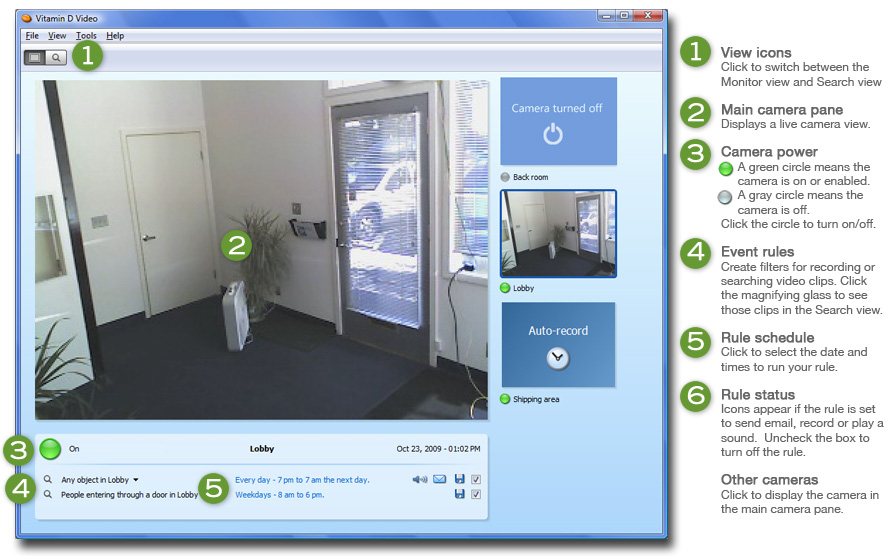
\includegraphics[width=4in]{figures/vitamind.jpg}
    \caption[Screen shot of Vitamin D Video.]{\small Screen shot of
      Vitamin D Video. Reprinted from the Vitamin D Video Web site
      (\url{http://www.vitamindinc.com/}).}
    \label{fig:vitamind}
  \end{center}
\end{figure}

It is interesting that Vitamin D Video does not use motion detection,
but rather uses people detection. It uses hierarchical temporal memory
(HTM; Hawkins, 2007)\nocite{jeff07htm} to detect people. This
algorithm attempts to apply the concept of how the brain recognizes a
person.

Video Analytics \shortcite{dvtel} is a video surveillance software
package that includes many different modules.  Sample modules are
intrusion detection, unattended baggage detection, object removal
detection, autonomous pan-tilt-zoom (PTZ) tracking, stopped vehicle
detection, loitering detection, and camera tampering
detection. However, some modules such as intrusion detection do not
have any intelligent features.

SuperTrack \shortcite{supertrack} is an intelligent video surveillance
system. SuperTrack is designed for automatically analyzing and
monitoring events without the need for human attention and
interaction. This system provides automatic object detection, abnormal
behavior detection, tracking, and so on. However, it requires the user
to configure and maintain a set of alarm trigger rules in
advance. SuperTrack also supports various types of cameras such as USB
cameras and network cameras.  Figure \ref{fig:supertrack} shows a
screen shot of the system.

\begin{figure}[t]
  \begin{center}
    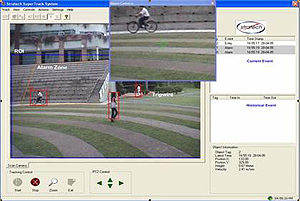
\includegraphics[width=3in]{figures/supertrack.jpg}
    \caption[Screen shot of SuperTrack.]{\small Screen shot of
      SuperTrack. Reprinted from the Stratech Web site
      (\url{http://www.stratechsystems.com/iv_supertrack.asp}).}
    \label{fig:supertrack}
  \end{center}
\end{figure}

\subsection{Summary}

Many open source and commercial video surveillance products are
available; however, most of them do not provide intelligent
features. Therefore, they cannot understand the events occurring in a
scene or learn human activities. In addition, users are required to
provide a great deal of configuration parameters before they can
deploy the system to operate in real-world situations. For instance,
in all of the systems, restricted zones or rules for a scene need to
be defined beforehand.

This review on open source and commercial video surveillance products
makes us realize the importance of and demand for human behavior
modeling and anomaly detection. Nowadays, in order to solve real-world
problems, research needs to focus on both academic issues and the
commercial market.

\section{Contributions}

The contributions of this dissertation are as follows.

\begin{enumerate}
  \item We propose an intelligent video surveillance system that is
    practical and fairly close to the ideal surveillance system, which
    should monitor and automatically raise alarms to security
    personnel;

  \item We develop an algorithm for extracting and tracking multiple 
    moving foreground blobs in a scene using an appearance model;

  \item We propose a shadow detection method that uses a simple
    maximum likelihood classification approach based on color
    information;

  \item We propose a new method for clustering human behaviors that 
    is suitable for bootstrapping an anomaly detection module for 
    intelligent video surveillance systems;

  \item We propose and develop a new and effective algorithm for
    semi-supervised learning of common human behaviors and detect 
    anomalies in video sequences;

  \item We introduce a new and more accurate algorithm for
    incrementally profiling human behaviors in video sequences without
    requiring storage of large databases of training data;

  \item We provide the source code and datasets
    online\footnote{See \url{http://www.kanouivirach.com/#downloads}.}
    for researchers interested in evaluating or extending our work.
\end{enumerate}

\subsection{List of Publications}

We provide a list of publications as part of this dissertation. We
also include the list of works currently under review and preparation
for submission.

\subsection*{Published Works}

\begin{itemize}
  \renewcommand\labelitemi{--} 

  \item \textbf{Clustering Human Behaviors with Dynamic Time Warping
    and Hidden Markov Models for a Video Surveillance
    System}\nocite{kan10clustering}\\ Kan Ouivirach and Matthew N.\
    Dailey\\ \textit{International Conference on Electrical
    Engineering/Electronics Computer Telecommunications and
    Information Technology (ECTI-CON)}, pages 884--888, 2010\\
    Publisher: IEEE Computer Society\\ Included in
    Chapter~\ref{ch:clustering}\\

  \item \textbf{Automatic Suspicious Behavior Detection from a Small
    Bootstrap Set}\nocite{kan12detection}\\ Kan Ouivirach, Shashi
    Gharti, and Matthew N.\ Dailey\\ \textit{International Conference
    on Computer Vision Theory and Applications (VISAPP)}, volume 1,
    pages 655--658, 2012\\ Publisher: Springer-Verlag\\ Included in
    Chapter~\ref{ch:batch}\\

  \item \textbf{Incremental Behavior Modeling and Suspicious Activity
    Detection}\nocite{kan13incremental}\\ Kan Ouivirach, Shashi
    Gharti, and Matthew N.\ Dailey\\ \textit{Pattern Recognition},
    46(3): 671--680, 2013\\ Publisher: Elsevier\\ Included in
    Chapter~\ref{ch:incremental}
  
\end{itemize}

\subsection*{Manuscripts Currently under Review}

\begin{itemize}
  \renewcommand\labelitemi{--}

  \item {\bf{Extracting the Object from the Shadows: Maximum
    Likelihood Object/Shadow Discrimination}}\\ Kan Ouivirach and
    Matthew N.\ Dailey\\ \textit{International Conference on
    Electrical Engineering/Electronics Computer Telecommunications and
    Information Technology (ECTI-CON)}, 2013\\ Publisher: IEEE
    Computer Society\\ Included in Chapter~\ref{ch:shadow}

\end{itemize}

\subsection*{Manuscripts Currently in Preparation}

\begin{itemize}
  \renewcommand\labelitemi{--}

  \item {\bf{Incorporating Geometric and Shadow Region Shape
    Information for Shadow Detection}}\\ Kan Ouivirach and Matthew N.\
    Dailey\\ To be submitted in \textit{International Conference on
    Computer Vision and Pattern Recognition (CVPR)}, 2013\\ Publisher:
    IEEE Computer Society

\end{itemize}

\section{Organization of Dissertation}

I organize the rest of this dissertation as follows.

In Chapter \ref{ch:blobanalysis}, I describe our blob-based motion
analysis methods including blob extraction and appearance-based blob
tracking.

In Chapter \ref{ch:shadow}, I present a new method for detecting
shadows using a simple maximum likelihood classification method based
on color information.

In Chapter \ref{ch:clustering}, I propose a new method for clustering
behaviors in a scene.

In Chapter \ref{ch:batch}, I present an automatic suspicious behavior
detection method that uses a small bootstrap set.

In Chapter \ref{ch:incremental}, I describe our extension of the
suspicious behavior detection approach for incremental learning in
which security personnel feedback is incorporated.

Finally, in Chapter \ref{ch:conclusion}, I conclude and discuss the
possible further extensions of my dissertation.

\FloatBarrier


% --- Maybe use later ---

%(see Figure \ref{fig:zm-console}) 
%\begin{figure}[t]
%  \begin{center}
%    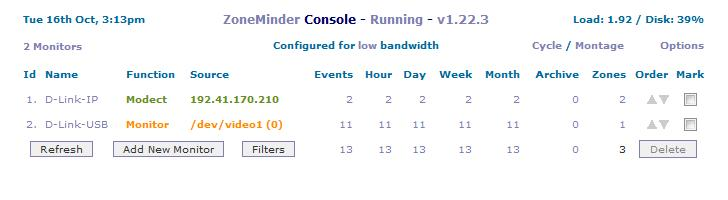
\includegraphics[width=4.5in]{figures/zm-console.jpg}
%    \caption{ZM Console} 
%    \label{fig:zm-console}
%  \end{center}
%\end{figure}

%ZM has three main modules. The first is the ZM Capture (ZMC) module
%whose job is to capture video frames from a video device as quickly as
%possible. The second is the ZM Analysis (ZMA) module, which performs
%video analysis. It finds the captured frames and checks whether the
%detected motion should generate an alarm or not. The last is the ZM
%Frame (ZMF) module. It is an optional module for writing the captured
%frames to file system. This module could potentially reduce the
%workload of ZMA, so ZMA can do more analysis work. If ZMF is not
%enabled, ZMA will write captured frames to file system instead.

%The core of ZM supports capturing and analyzing images. It also
%provides a configurable set of parameters (see
%Figure \ref{fig:zm-option}). ZM allows us to define ``zones'' for each
%camera and vary the sensitivity and functionality (see
%Figure \ref{fig:zm-webcam01-zones}
%and \ref{fig:zm-webcam01-zones-define}). Therefore, we can eliminate
%unnecessary regions and set the different thresholds for each zone. ZM
%also provides a motion detection feature for detecting changes in a
%scene and setting an alarm based on the user-defined threshold.

%\begin{figure}[t]
%  \begin{center}
%    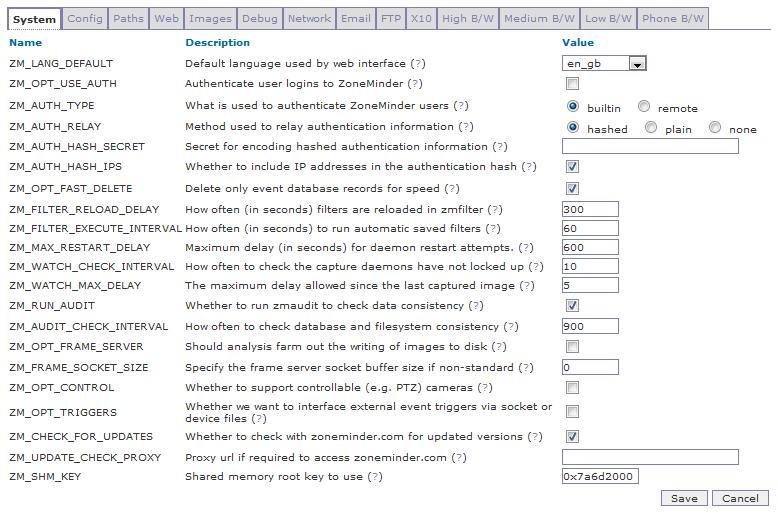
\includegraphics[width=4.5in]{figures/zm-options.jpg}
%    \caption{ZM Options}
%    \label{fig:zm-option}
%  \end{center}
%\end{figure}

%\begin{figure}[t]
%  \begin{center}
%    \subfloat[]{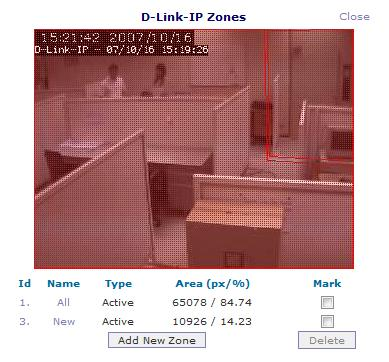
\includegraphics[scale=0.5]{figures/zm-webcam01-zones.jpg}\label{fig:zm-webcam01-zones}}
%    \hspace{0.1in}
%    \subfloat[]{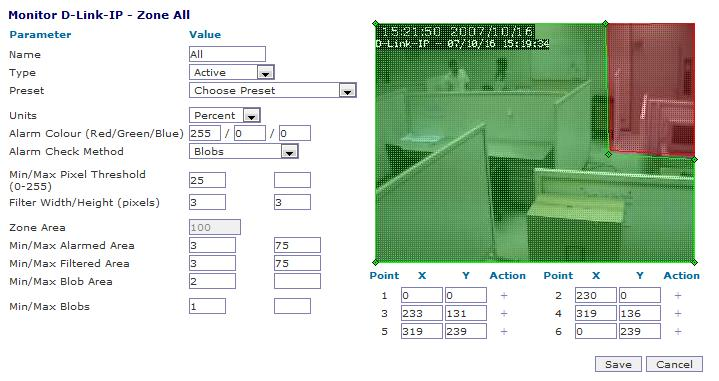
\includegraphics[scale=0.5]{figures/zm-webcam01-zones-define.jpg}\label{fig:zm-webcam01-zones-define}}
%  \end{center}  
%  \caption[Example of zone defined in ZoneMinder]{Example of (a) zone
%  defined and (b) configuring a zone in ZoneMinder.}
%  \label{fig:zm-webcam-zones}
%\end{figure}

%Here I review only the intrusion detection module.  
%The intrusion detection module automatically detects prohibited
%intrusion behaviors while ignoring distractions that cause false
%alarms, like small animals, swaying branches,
%etc. Figure \ref{fig:intrusion-detection} shows a screen shot of the
%result from this module. This module can be used on stationary cameras
%as well as on PTZ cameras. There are two modes which are Regional
%Entrance and Tripwire. The first mode provides a security alarm when
%the system detects a person or vehicle moving within a prohibited
%area. The second mode provides a security alarm when a person or
%vehicle breaks through a demarcation line. User can configure this
%mode to prohibit any crossover or to allow movement in a single
%direction.

%\begin{figure}[t]
%  \begin{center}
%    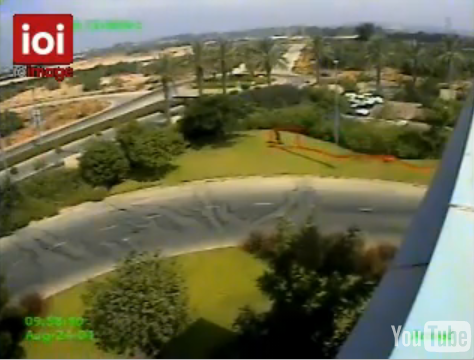
\includegraphics[width=3in]{figures/intrusion-detection.png}
%     \caption[Screen shot of DVTel's intrusion detection
%     module]{Screen shot of DVTel's intrusion detection
%     module. Captured from the video demonstration on DVTel's Web
%     site.}
%    \label{fig:intrusion-detection}
%  \end{center}
%\end{figure}

%For example, it has the knowledge that a head contains two
%eyes and a mouth; so, if either an eye or mouth is detected, it will
%assume that there is a head at that position. Vitamin D Video trained
%a learning network with several hundred videos of humans. Also,
%examples of vehicles and animals not people are trained. As a result,
%Vitamin D Video can tolerate to real world problems.
